%%%%%%%%%%%%%%%%%%%%%%%%%%%%%%%%%%%%%%%%%%%%%%%%%%%%%%%%%%%%%%%%%
%
% Project     : Bachelorarbeit
% Title       : Machbarkeitsanalyse für eine ressourcenorientierte Schnittstelle zur Verarbeitung grundlegender Probleme der Informatik
% File        : probleme.tex Rev. 01
% Date        : 01.03.2015
% Author      : Raffael Santschi
%
%%%%%%%%%%%%%%%%%%%%%%%%%%%%%%%%%%%%%%%%%%%%%%%%%%%%%%%%%%%%%%%%%

\chapter{Analyse und Auswahl der Probleme}\label{chap.problemauswahl}
In diesem Kapitel werden verschiedene Probleme und das dazugehörige Auswahlverfahren erläutert, welche für die Erstellung der Schnittstelle betrachtet wurden.

\section{Auswahl der Probleme}\label{cat_theo_inf}
Da es in der Welt unzählige Probleme mit hoher Laufzeitkomplexität gibt, musste ein geeignetes Verfahren ausgefunden werden, mit dem verschiedene Typen dieser Probleme für die Schnittstelle evaluiert werden konnten. In \cite{garey1979computers} werden verschiedene NP-vollständige und NP-schwere Probleme vorgestellt. Diese werden in Kategorien unterteilt (siehe Aufzählung unten), welche in dieser Arbeit ebenfalls benutzt werden.

\begin{itemize}
	\item Graphentheorie
	\item Netzwerk Design
	\item Sets und Partitionen
	\item Speicher und Wiederherstellung
	\item Sequenzierung und Planung
	\item Mathematisches Programmieren
	\item Algebra und Zahlentheorie
	\item Spiele und Puzzles
	\item Logik
	\item Automaten und Sprachtheorie
	\item Programm Optimierung
	\item Sonstiges
	\item Offene Probleme
\end{itemize}

Im Rahmen dieser Arbeit konnten nicht alle Probleme angeschaut werden, deshalb wurde geschaut, ob es Probleme gibt, welche in der Realität auftreten und nicht nur rein wissenschaftliche Probleme sind. Aus diesen Problemen wurden dann fünf ausgewählt, bei der Auswahl wurde auch geschaut, dass die Probleme zum grossen Teil aus unterschiedlichen Kategorien kommen, jedoch wurden auch zwei aus der gleichen Kategorie ausgewählt. Die ausgewählten Probleme werden im folgenden Abschnitt genauer erläutert und für die weiteren Schritte der Erstellung der Schnittstelle berücksichtigt. Durch dieses Vorgehen konnte eine hohe Diversität von Problemen sichergestellt werden, was bei der Erstellung der Anforderungen und Architetkur hilfreich war.

\subsection{Hierarchie der Reduktion}\label{hierarchy_reduction}
Wie bereits in der Einleitung beschrieben, muss für den Beweis der NP-Vollständigkeit ein bekanntes NP-vollständiges Problem auf das Bestehende reduziert werden können. In \autoref{fig:hierarchy_reduction} ist die Hierarchie bis zu den ausgewählten Problemen aufgezeigt.

\begin{figure}[h]
\centering 
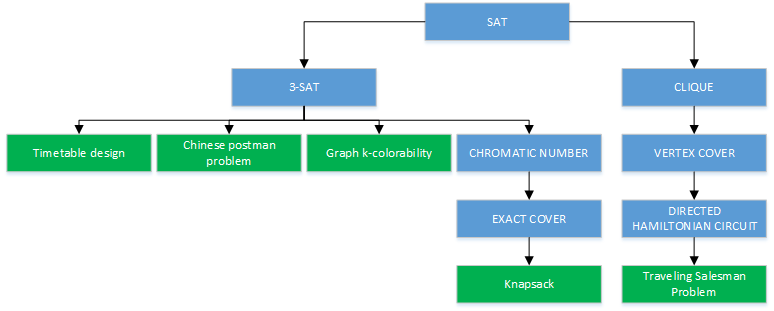
\includegraphics[scale=0.8]{images/visio/problem_hierarchy.png}
\caption{Hierarchie der Reduktion zum Beweis der NP-Vollständigkeit}
\label{fig:hierarchy_reduction}
\end{figure}

\newpage
\subsection{Graphentheorie}\label{graph_theory}

	\subsubsection{Färbung (Graphtheorie)}\label{colarability_graph_theory}
	Die Färbung in der Graphtheorie ist ein NP-vollständiges Problem. Dies wurde durch die Reduktion des 3-SAT Problemes bewiesen.

	\paragraph{Beschreibung}
	Englischer Name: Graph k-colorability

	Bei diesem Problem geht es darum die Knoten eines Graphens so zu färben, dass keine zwei benachbarten Knoten die gleiche Farbe tragen. Ein Graph heisst k-färbbar, wenn die Färbung mit k Farben korrekt durchgeführt werden kann. Dieses Problem ist für $k = 2$ in polynomieller Zeit lösbar, für $k \ge 2$ jedoch nicht mehr, dies jedoch auch nur mit gewiesen Einschränkungen (siehe \cite{garey1979computers}).

	\paragraph{Beispiel}
	Gegeben sei ein Graph mit 10 Knoten mit einer vorgegebenen Konfiguration (siehe \autoref{fig:graph_faerbung}).\\
	Gesucht ist die Färbung der Knoten, damit keine zwei benachbarten Knoten die gleiche Farbe haben, bzw. die minimale Anzahl Farben ($k$), welche verwendet werden müssen, damit die Bedingung erfüllt ist. Der Graph \ref{fig:graph_faerbung_incorrect} zeigt eine ungültige Lösung mit zwei Farben. Durch einen Algorithmus kann ermittelt werden, dass dieser Graph mindestens drei Fraben (siehe \ref{fig:graph_faerbung_correct}) benötigt, um die Bedingung zu erfüllen. Somit ist $k=3$.
\begin{figure}[ht]
\centering
\subfigure[Inkorrekte Färbung]{
  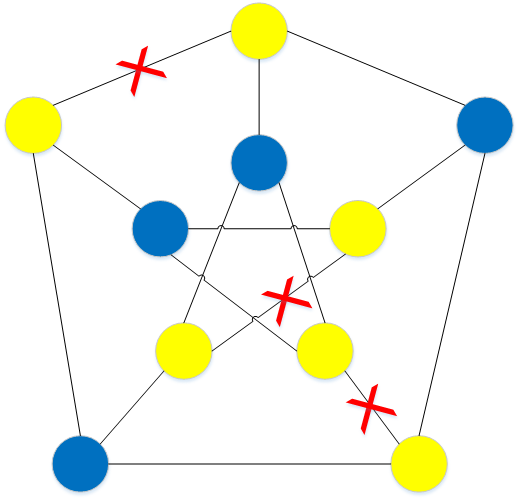
\includegraphics[scale=0.5]{images/visio/graph_faerbung_incorrect.png}
  \label{fig:graph_faerbung_incorrect}
}
\subfigure[Korrekte Färbung]{
  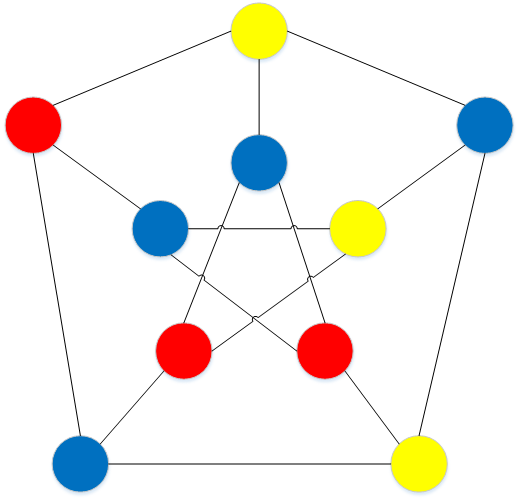
\includegraphics[scale=0.5]{images/visio/graph_faerbung_correct.png}
  \label{fig:graph_faerbung_correct}
}
\label{fig:graph_faerbung}
\caption{Kanten Färbung eines Graphen mit 10 Knoten}
\end{figure}

	\paragraph{Eingabe- und Ausgabedaten}\mbox{}\\
	Eingabedaten: Knoten mit ihren Verbindungen zu anderen Knoten\\
	Ausgabedaten: Knoten mit ihrer Färbung und $k$ (Anzahl benötigter Farben)

	\paragraph{Bekannte Algorithmen}
	(siehe \cite{seminar_algo_graph}, \cite{krumke2012graphentheoretische} und \cite{seminar_rob_graphen})
	\begin{itemize}
		\item Spalten-Generierungs-Ansatz
		\item Sequentielles Färben (Sequential Coloring)
		\item \intromark{Backtracking Algorithmus}
		\item \intromark{Greedy Algorithmus}
		\item Johnson-Algorithmus
	\end{itemize}	

	\paragraph{Bekannte reale Probleme}	
	Es gibt diverse reale Probleme, welche mit der Knotenfärbung gelöst werden können, hier sind nur einige davon aufgelistet:
	\begin{itemize}
		\item Stundenplan: Anhand der eingegebenen Daten wird ein Konfliktmatrix erstellt und diese dann in ein Färbungsproblem umgewandelt. Die Anzahl benötigten Farben sind dann die Anzahl der verschiedenen Perioden, welche es benötigt, um eine Stundenplan ohne Konflikte zu erstellen. \cite{ieee_exam_table_graph_coloring} \cite{time_table_graph_coloring}
		\item Frequenzverteilung (Mobilfunk): Im Mobilfunkt hat jede Antenne einen Frequenzbereich, im Graph werden die Antennen miteinander verwunden, bei denen die Reichweite überschneidet. Den Farben kann dann eine Frequenz zu gewiesen werden und das Resultat ist eine Konfliktfreie Mobilnetzabdeckung. \cite{seminar_rob_graphen}
		\item Färben von Landkarten: Die Länder sind die Knoten, die Kanten die Verbindung zu den Nachbarländern und die erreichnete Farbe ist die Einfärbung auf der Landkarte. \cite{seminar_rob_graphen}
	\end{itemize}

\newpage
\subsection{Netzwerk Design}\label{network_design}

	\subsubsection{Problem des Handlungsreisenden}\label{tsp}
	Das Problem des Handlungsreisenden ist ein NP-vollständiges Problem. Dies wurde durch die Reduktion des Hamiltonkreisproblemes bewiesen. \todo{evtl. Umbennenung Rundreiseproblem}

	\paragraph{Beschreibung}
	Englischer Name: Traveling Salesman Problem\\
	Beim Problem des Handlungsreisenden geht es darum mit einer optimalen Route von einem Ausgangspunkt verschiedene Wegpunkte abzufahren und wieder zum Ausgangspunkt zurück zu kehren. Es gibt verschiedene Ausprägungen des Problems, es kann zum Beispiel bestimmt werden, dass die Verbindung zwischen zwei Punkten hin und zurück gleich lang sind, was die Komplexität halbiert. Mit der Erhöhung der Anzahl Wegpunkte nimmt die Komplexität mit $O(n!)$ zu. Bei zehn Wegpunkten und ungleichen Hin- und Zurückwege sind das bereit über dreieinhalb Millionen Möglichkeiten.

	\paragraph{Beispiel} Gegeben seien vier Wegpunkte (A, B, C, D), der Startpunkt sei A.\\
	Gesucht ist die optimale Route, welche alle Wegpunkte beinhaltet und wieder bei A endet.\\
	Die Abbildung \ref{fig:tsp_example} zeigt alle möglichen Lösung mit ihren errechneten Werten. Die Route A-D-C-B-A ist mit einem Wert von 16 die beste Route. Weiter ist zu sehen, dass schon bei 4 Wegpunkten 6 Möglichkeiten vorhanden sind.
\begin{figure}[h]
\centering
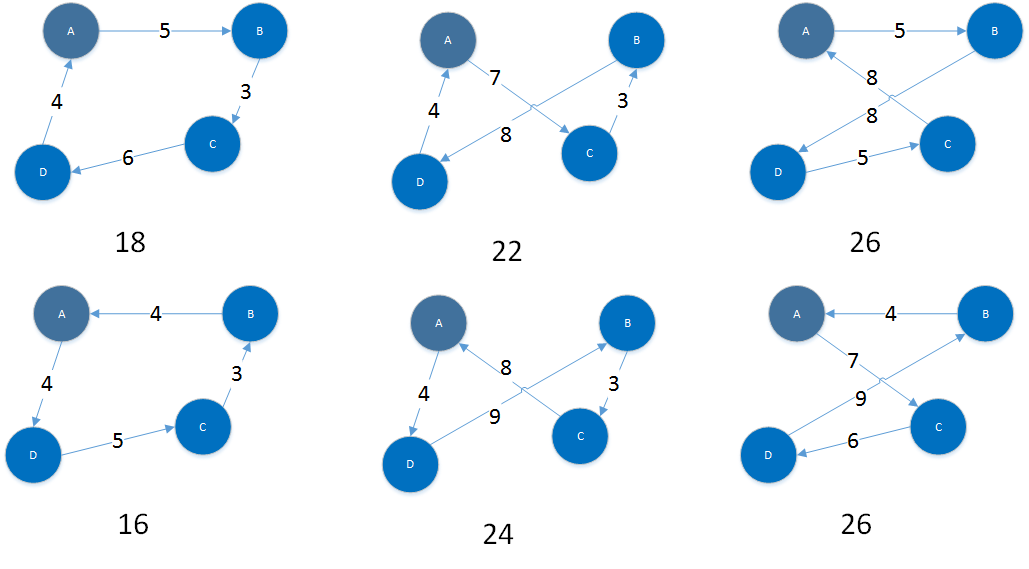
\includegraphics[scale=0.6]{images/visio/tsp.png}
\caption{Problem des Handlungsreisenden mit 4 Wegpunkten}
\label{fig:tsp_example}
\end{figure}

	\paragraph{Eingabe- und Ausgabedaten}\mbox{}\\
	Eingabedaten: Startpunkt und Wegpunkte, welche passiert werden müssen\\
	Ausgabedaten: Reihenfolge der Wegpunkte für eine optimale Route

	\paragraph{Bekannte Algorithmen}\cite{tsp_algorithmen} \cite{tsp_semesterarbeit}
	\begin{itemize}
		\item Nearest-Neighbor
		\item 2Opt
		\item Christofides
	\end{itemize}

	\subsubsection{Briefträgerproblem}\label{chinese_postman}
	Das Briefträgerproblem ist ein NP-vollständiges Problem. Dies wurde durch die Reduktion des 3-SAT Problemes bewiesen.

	\paragraph{Beschreibung}
	Englischer Name: Chinese postman problem\\
	Das Briefträgerproblem ist ähnlich wie das Problem des Handlungsreisenden, jedoch geht es darum jede Kante mindestens ein Mal abzufahren. Die Knoten stellen Kreuzungen dar, die Kanten sind Strassen. Die minimale Länge kann mit Hilfe des \glossarmark{Eulerischenkreises} relativ einfach berechnet werden. Falls der Graph die Kriterien des \glossarmark{Eulerischenkreises} nicht erfüllt, werden alle Knoten mit ungeraden Anzahl von Kanten mit einem anderen solchen Knoten über die kürzeste Route verbunden werden. Die minimal Läng ist dann alle Strecke und die Hilfsstrecken zusammen gezählt.
	\cite{pearson2004decision}

	\paragraph{Beispiel} Gegeben sei der Graph mit den Punkten A bis H und den blau eingezeichneten Verbindungen.\\
Gesucht ist eine Route mit dem kürzesten Weg, welche jede Kante mindestens ein Mal abfährt. \cite{pearson2004decision}\\
Die grün eingezeichneten Verbindungen sind Hilfslinien, um den Graph in einen \glossarmark{Eulerischenkreis} zu verwandeln. Eine mögliche Lösung mit der minimal Länge von 1000 ist die Route A-D-C-G-H-C-A-B-D-F-B-E-F-H-F-B.
\begin{figure}[h]
\centering
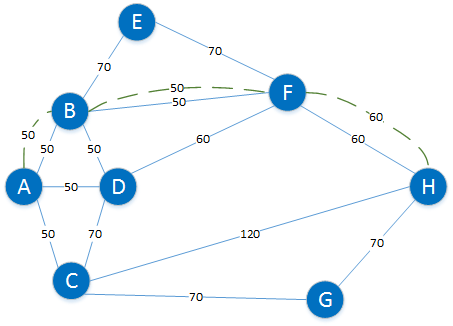
\includegraphics[scale=0.8]{images/visio/chinese_postman.png}
\caption{Beispiel für ein Briefträgerproblem}
\label{fig:chinese_postman_example}
\end{figure}

	\paragraph{Eingabe- und Ausgabedaten}\mbox{}\\
	Eingabedaten: Startpunkt und Knoten mit ihren Verbindungen zu anderen Knoten\\
	Ausgabedaten: Reihenfolge der Knoten für eine minimale Strecke

	\paragraph{Bekannte Algorithmen}\mbox{}\\
	Briefträgeralgorithmus (Chinese postman algorithm)

\subsection{Sequenzierung und Planung}\label{sequencing_scheduling}

	\subsubsection{Stundenplan Design}\label{tsp}
	Das Erstellen eines Stundenplanes ist ein NP-vollständiges Problem. Dies wurde durch die Reduktion des 3-SAT Problemes bewiesen.

	\paragraph{Beschreibung}
	Englischer Name: Timetable design\\
	Die Erstellung von Stundenplänen ist ein sehr komplexes Problem, basierend auf Fächer, Lehrer, Klassen und Klassenzimmern wird versucht eine optimale Verteilung der Stunden zu erreichen. Die wichtigste Bedingung (hard constraints) ist, dass ein Lehrer zur selben Zeit nur jeweils 1 Fach unterrichtet und für die Klasse und das Klassenzimmer gilt dasselbe. Zusätzlich gibt es dann noch beliebig weitere Kriterien (soft constraints), wie zum Beispiel das eine Klasse nie mehr als 9 Lektionen pro Tag haben soll oder ein Lehrer nie mehr als 5 Lektionen am Stuck unterrichten sollte. Bei der Erstellung von Stundenplänen spricht man von hard constraints und soft constraints. Ein hard constraint ist im Gegensatz zu eine soft constraint unabdingbar, das heisst, es ist nicht möglich, dass ein Lehrer zwei verschiedene Fächer gleichzeitig unterrichtet, jedoch könnte er mehr als 5 Lektionen hintereinander unterrichten. \cite{Abramson92aparallel} \cite{Abramson91constructingschool} \cite{framework_timetabling} \cite{time_table_constraint_opti_ea}

	\paragraph{Beispiel} Gegeben seien die Fächer, Lehrer, Klassen und Klassenzimmer aus den Tabellen \ref{table:eg_subject}, \ref{table:eg_teacher}, \ref{table:eg_schoolclasses} und \ref{table:eg_schoolroom}.\\
Gesucht ist ein Stundenplan, bei welchem es keine Kollisionen für Lehrer, Klassen und Klassenzimmer gibt.

\begin{table}[ht]
\centering
  \begin{tabular}{ l | l }
	\hline
	\rowcolor{gray}
	\textbf{Fachname}	& \textbf{Kürzel}\\ \hline
	Mathematik		& M\\ \hline
	Deutsch		& D\\ \hline
	Englisch		& E\\ \hline
	Französisch		& F\\ \hline
	Sport			& Sp
  \end{tabular}
   \caption{Schulfächer}\label{table:eg_subject}
\end{table}

\begin{table}[ht]
\centering
  \begin{tabular}{ l | l }
	\hline
	\rowcolor{gray}
	\textbf{Lehrername} 	& \textbf{Ausbildung}\\ \hline
	Angst				& Deutsch, Mathematik, Sport\\ \hline
	Arm				& Sport\\ \hline
	Bernasconi			& Deutsch, Mathematik, Französisch\\ \hline
	Müller				& Deutsch, Mathematik, Englisch, Französisch\\ \hline
	Pfister				& Englisch, Franszösisch
  \end{tabular}
   \caption{Lehrer}\label{table:eg_teacher}
\end{table}

\begin{table}[ht]
\centering
  \begin{tabular}{ l | l }
	\hline
	\rowcolor{gray}
	\textbf{Klassenname} 	& \textbf{Benötigte Fächer}\\ \hline
	Tja13				& Deutsch, Mathematik, Sport\\ \hline
	Tja12				& Deutsch, Mathematik, Sport, Französisch\\ \hline
	Tja11				& Deutsch, Mathematik, Sport, Französisch, Englisch\\ \hline
	Tja10				& Deutsch, Mathematik, Sport, Französisch, Englisch
  \end{tabular}
   \caption{Klassen}\label{table:eg_schoolclasses}
\end{table}

\begin{table}[ht]
\centering
  \begin{tabular}{ l }
	\hline
	\rowcolor{gray}
	\textbf{Fachname}\\ \hline
	Zimmer 101\\ \hline
	Zimmer 103\\ \hline
	Zimmer 201\\ \hline
	Turnhalle
  \end{tabular}
   \caption{Klassenzimmer}\label{table:eg_schoolroom}
\end{table}

\FloatBarrier
In der \autoref{table:timetable_1} sieht man eine mögliche Lösung zu dieser Problemstellung, dabei wurde beachtet, dass die Lehrer möglichst gleich viele Stunden unterrichten und die Schüler keine doppelten Freistunden haben. Es ist jedoch auffällig, dass das Zimmer 201 sehr schlecht ausgenützt ist, in der zweiten Variante (siehe \autoref{table:timetable_2}), wurden die Stunden der Klasse Tja11 so verschoben, dass das Zimmer 201 nicht mehr benötigt wird. Das hat jedoch zur Folge, dass die Klasse Tja11 nun eine doppelte Freistunde hat. Die Eingabedaten sind in diesem Beispiel noch sehr überschaubar, doch es gibt schon bereits enorm viele verschiedenen Möglichkeite und Ausprägungen.

\begin{table}[ht]
\centering
  \begin{tabular}{ l | l | l | l | l }
	\hline
	\rowcolor{gray}
	\textbf{Uhrzeit} 	& \textbf{Turnhalle}	& \textbf{Zimmer 101} 	& \textbf{Zimmer 103}	&  \textbf{Zimmer 201}\\ \hline
	0800-0900		& Sp / Tja13 / Arm		& D / Tja11 / Müller		& 				& \\ \hline
	0900-1000		& Sp / Tja13 / Arm		& M / Tja11 / Müller		& F / Tja12 / Pfister		& \\ \hline
	1000-1100		& Sp / Tja12 / Arm		& D / Tja10 / Bernasconi	& M / Tja13 / Angst		& F / Tja11 / Müller\\ \hline
	1100-1200		& Sp / Tja12 / Arm		& M / Tja10 / Angst		& D / Tja13 / Bernasconi	& E / Tja11 / Pfister\\ \hline \hline
	1300-1400		& Sp / Tja11 / Angst	& F / Tja10 / Bernasconi	& D / Tja12 / Müller		& \\ \hline
	1400-1500		& Sp / Tja11 / Angst	& E / Tja10 / Pfister		& M / Tja12 / Bernasconi	& \\ \hline
	1500-1600		& Sp / Tja10 / Angst	& 				& 				& \\ \hline
	1600-1700		& Sp / Tja10 / Angst	& 				& 				& \\ \hline
  \end{tabular}
   \caption{Möglicher Stundenplan - Variante 1}\label{table:timetable_1}
\end{table}

\begin{table}[ht]
\centering
  \begin{tabular}{ l | l | l | l }
	\hline
	\rowcolor{gray}
	\textbf{Uhrzeit} 	& \textbf{Turnhalle}	& \textbf{Zimmer 101} 	& \textbf{Zimmer 103}	\\ \hline
	0800-0900		& Sp / Tja13 / Arm		& D / Tja11 / Müller		& 				\\ \hline
	0900-1000		& Sp / Tja13 / Arm		& M / Tja11 / Müller		& F / Tja12 / Pfister		\\ \hline
	1000-1100		& Sp / Tja12 / Arm		& D / Tja10 / Bernasconi	& M / Tja13 / Angst		\\ \hline
	1100-1200		& Sp / Tja12 / Arm		& M / Tja10 / Angst		& D / Tja13 / Bernasconi	\\ \hline \hline
	1300-1400		& Sp / Tja11 / Angst	& F / Tja10 / Bernasconi	& D / Tja12 / Müller		\\ \hline
	1400-1500		& Sp / Tja11 / Angst	& E / Tja10 / Pfister		& M / Tja12 / Bernasconi	\\ \hline
	1500-1600		& Sp / Tja10 / Angst	& F / Tja11 / Müller		& 				\\ \hline
	1600-1700		& Sp / Tja10 / Angst	& E / Tja11 / Pfister		& 				\\ \hline
  \end{tabular}
   \caption{Möglicher Stundenplan - Variante 2}\label{table:timetable_2}
\end{table}

\FloatBarrier
	Eine sehr gut ausgearbeitete Software ist 'Units' \cite{unit_express}, sie liefert umfangreiche Funktionen zur Erstellung von Stundenplänen und hat einen sehr ausgeklügelten Optimierungsalgorithmus.

	\paragraph{Eingabe- und Ausgabedaten}\mbox{}\\
	Eingabedaten: Fächer, Lehrer, Klassen und Klassenzimmer mit verschiedenen Einschränkungen und Zusatzinformationen\\
	Ausgabedaten: Einteilung der Fächer mit den dazugehörigen Klassen, Lehrern und Zimmer auf verschiedene Tage und Uhrzeiten, welche keine Konflikte enthält

	\paragraph{Bekannte Algorithmen}
	(siehe \cite{framework_timetabling})
	\begin{itemize}
		\item \intromark{Backtracking Algorithmus}
		\item \intromark{Evolutionäre Algorithmen}
		\item Constraint Logic Programming
	\end{itemize}	

	\paragraph{Bekannte ähnliche Probleme}	
	Es gibt diverse andere Planungsprobleme, welche auf dem gleichen Konzept basieren, jedoch unterschiedliche Eingabedaten und Beschränkungen haben:
	\begin{itemize}
		\item Spielplan
		\item Prüfungsplan
		\item Schichtenplanung
	\end{itemize}

\newpage
\subsection{Mathematisches Programmieren}\label{mathematical_programming}

	\subsubsection{Rucksack Problem}\label{knapsack}
	Das Rucksack Problem ist ein NP-vollständiges Problem. Dies wurde durch die Reduktion des Problemes der exakten Überdeckung bewiesen.

	\paragraph{Beschreibung}
	Englischer Name: Knapsack\\
	Beim Rucksack Problem geht es um einen Container, symbolisch der Rucksack, mit einer Gewichtsschranke, desweiteren gibt es noch Objekte, welche in den Container gepackt werden können. Diese Objekte besitzen ein Gewicht und einen Profit. Das Ziel ist es den grösst möglichen Profit zu erlangen, ohne die Gewichtsschranke zu überschreiten. \cite{knapsack_desc_web}

	\paragraph{Beispiel} Gegeben sei ein Rackete mit der Gewichtsschranke 645kg und die Objekte in Tabelle \ref{table:knapsack_objects}.\\
Gesucht ist die Objektauswahl mit dem grössten Profit, welche die Gewichtsschranke nicht überschreitet.\\
In diesem Beispiel wäre die optimale Lösung 1, 2, 3 und 5. \cite{knapsack_desc_web}

\begin{table}[ht]
\centering
  \begin{tabular}{ c | r | r }
	\hline
	\rowcolor{gray}
	\textbf{Objekt-Nr.}	&	\textbf{Gewicht in kg}	&	\textbf{Profit}\\ \hline
	1			&	153			&	232\\ \hline
	2			&	54			&	73\\ \hline
	3			&	191			&	201\\ \hline
	4			&	66			&	50\\ \hline
	5			&	239			&	141\\ \hline
	6			&	137			&	79\\ \hline
	7			&	148			&	48\\ \hline
	8			&	249			&	38
  \end{tabular}
   \caption{Knapsack Objekte mit Gewicht und Profit}\label{table:knapsack_objects}
\end{table}

	\paragraph{Eingabe- und Ausgabedaten}\mbox{}\\
	Eingabedaten: Gewichtsschranke und Elemente mit Gewicht und Nutzwert\\
	Ausgabedaten: Zusammenstellung von den Elementen mit höchstem Nutzwert

	\paragraph{Bekannte Algorithmen}
	\begin{itemize}
		\item \intromark{Backtracking Algorithmus}
		\item \intromark{Greedy Algorithmus}
		\item Algorithmus von Nemhauser und Ullmann \cite{knapsack_desc_web}
	\end{itemize}	

	\paragraph{Bekannte reale Probleme}	
	Es gibt diverse reale Probleme, welche mit der dem Rucksack Problem gelöst werden können \cite{kellerer2004knapsack}, hier sind nur einige davon aufgelistet:
	\begin{itemize}
		\item Ausschneiden von verschiedenen Stücken aus einem grossen Stück Metal oder Holz: Optimale Nutzung der Fläche(n), damit am Schluss genug Einzelstücke für das Herstellen des Endprodukt vorhanden sind.
		\item Kreditvergabe: Optimale Ausnutzung des Kreditbudget mit der Vergabe von Krediten an Kunden, welche eine Kredit über eine gewisse Höhe haben möchte und eine bestimmte Risikoeinstufung haben.
	\end{itemize}


\newpage
\subsection{Logik}\label{logic}
Die hier aufgeführten Probleme sind nur zur Vollständigkeit aufgelistet und beschrieben, sie werden nicht für die weiteren Schritte der Schnittstelle verwendet. Sie sind die Grundpfeiler der NP-Vollständigkeit, durch sie konnten zahlreiche Probleme als NP-schwer oder NP-vollständig deklariert werden.

	\subsubsection{Erfüllbarkeitsproblems der \glossarmark{Aussagenlogik} (SAT)}\label{sat}
	Das Erfüllbarkeitsproblem der Aussagenlogik ist ein NP-vollständiges Problem. Dies wurde durch Stephen A. Cook in den 1970er Jahre bewiesen \cite{cook_complexity}.

	\paragraph{Beschreibung}
	Englischer Name: Satisfiability (SAT)\\
	Beim Erfüllbarkeitsproblem der \glossarmark{Aussagenlogik} geht es darum zu überprüfen, ob eine beliebige aussagenlogische Formel erfüllbar ist.	

	\paragraph{Beispiel} Gegeben sei eine aussagenlogische Formel \ref{eq:aussagenlogik}.\\
	Gesucht ist die Antwort auf die Erfüllbarkeit dieser Formel.\\
	In der Tabelle \ref{table:sat_results} kann man sehen, dass die Formel erfüllbar ist, nämlich für die Kombinationen 3, 4 und 8.

	\begin{equation}
   		(A \vee B) \wedge C
  		 \label{eq:aussagenlogik}
	\end{equation}

\begin{table}[ht]
\centering
  \begin{tabular}{ c | c | c | c | c | c}
	\hline
	\rowcolor{gray}
	\textbf{Kombination-Nr.}	&	\textbf{A}	&	\textbf{B} 	& 	\textbf{C} 	&	$A \vee B$	&	\textbf{Resultat}\\ \hline
	1			&	wahr	& 	falsch	& 	falsch	&	wahr		&	falsch\\ \hline
	2			&	wahr	& 	wahr	& 	falsch	&	wahr		&	falsch\\ \hline
	\textbf{3}		&	wahr	& 	falsch	& 	wahr	&	wahr		&	\textbf{wahr}\\ \hline
	\textbf{4}		&	wahr	& 	wahr	& 	wahr	&	wahr		&	\textbf{wahr}\\ \hline
	5			&	falsch	& 	falsch	& 	falsch	&	falsch		&	falsch\\ \hline
	6			&	falsch	& 	wahr	& 	falsch	&	wahr		&	falsch\\ \hline
	7			&	falsch	& 	falsch	& 	wahr	&	falsch		&	falsch\\ \hline
	\textbf{8}		&	falsch	& 	wahr	& 	wahr	&	wahr		&	\textbf{wahr}\\ \hline
  \end{tabular}
   \caption{Wahrheitstabelle zur aussagenlogischen Formel}\label{table:sat_results}
\end{table}

\newpage
	\subsubsection{3-SAT}\label{3sat}
	Das 3-SAT Problem ist ein NP-vollständiges Problem. Dies wurde durch die Reduktion des SAT Problemes bewiesen.

	\paragraph{Beschreibung}
	Englischer Name: 3-Satisfiability (3-SAT)\\
	Das 3-SAT Problem ist eine Spezialfall des SAT Problems, es dürfen maximal 3 Literale in einer Klausel enthalten sein.

	\paragraph{Beispiel} Gegeben sei eine 3-SAT Formel \ref{eq:aussagenlogik_3sat}.\\
	Gesucht ist die Antwort auf die Erfüllbarkeit dieser Formel.\\
	In der Tabelle \ref{table:3sat_results} kann man sehen, dass die Formel erfüllbar ist, lediglich für die Kombinationen 5, 11, 13 und 15 ist sie nicht korrekt.

	\begin{equation}
   		(A \wedge B \wedge C) \vee (B \wedge \neg C \wedge D)
  		 \label{eq:aussagenlogik_3sat}
	\end{equation}

\begin{table}[ht]
\centering
  \begin{tabular}{ c | c | c | c | c | c | c | c}
	\hline
	\rowcolor{gray}
	\textbf{Kombination-Nr.}	& \textbf{A}	& \textbf{B} 	& \textbf{C} & \textbf{D}  & $A \wedge B \wedge C$ & $B \wedge \neg C \wedge D$	& \textbf{Resultat}\\ \hline
	\textbf{1}			& wahr	& falsch	& falsch	& wahr	& wahr			 & wahr				& \textbf{wahr}\\ \hline
	\textbf{2}			& wahr	& wahr	& falsch	& wahr	& wahr			 & wahr 				& \textbf{wahr}\\ \hline
	\textbf{3}			& wahr	& falsch	& wahr	& wahr	& wahr			 & wahr				& \textbf{wahr}\\ \hline
	\textbf{4}			& wahr	& wahr	& wahr	& wahr	& wahr			 & wahr				& \textbf{wahr}\\ \hline
	5				& falsch	& falsch	& falsch	& wahr	& falsch			 & wahr				& falsch\\ \hline
	\textbf{6}			& falsch	& wahr	& falsch	& wahr	& wahr			 & wahr				& \textbf{wahr}\\ \hline
	\textbf{7}			& falsch	& falsch	& wahr	& wahr	& wahr			 & wahr 				& \textbf{wahr}\\ \hline
	\textbf{8}			& falsch	& wahr	& wahr	& wahr	& wahr			 & wahr 				& \textbf{wahr}\\ \hline
	\textbf{9}			& wahr	& falsch	& falsch	& falsch	& wahr			 & wahr				& \textbf{wahr}\\ \hline
	\textbf{10}			& wahr	& wahr	& falsch	& falsch	& wahr			 & wahr 				& \textbf{wahr}\\ \hline
	11				& wahr	& falsch	& wahr	& falsch	& wahr			 & falsch				& falsch\\ \hline
	\textbf{12}			& wahr	& wahr	& wahr	& falsch	& wahr			 & wahr				& \textbf{wahr}\\ \hline
	13				& falsch	& falsch	& falsch	& falsch	& falsch			 & wahr				& falsch\\ \hline
	\textbf{14}			& falsch	& wahr	& falsch	& falsch	& wahr			 & wahr				& \textbf{wahr}\\ \hline
	15				& falsch	& falsch	& wahr	& falsch	& wahr			 & falsch 				& falsch\\ \hline
	\textbf{16}			& falsch	& wahr	& wahr	& falsch	& wahr			 & wahr 				& \textbf{wahr}\\ \hline
  \end{tabular}
   \caption{Wahrheitstabelle zur 3-SAT Formel}\label{table:3sat_results}
\end{table}




